\begin{frame}{the one-way bridge}
\begin{tikzpicture}
\tikzset{
    bridge line/.style={ultra thick},
    road divide/.style={very thick,loosely dashed},
    old car black/.pic={
        \node at (0,-0.25) {
\includegraphics[width=1.25cm,angle=-90,origin=c]{../deadlock/Car_icon_top.pdf}};
    },
    old car black opposite/.pic={
        \node at (0,-0.25) {
\includegraphics[width=1.25cm,angle=90,origin=c]{../deadlock/Car_icon_top.pdf}};
    },
    old car black opposite rot/.pic={
        \node at (0,-0.25) {
\includegraphics[width=1.25cm,angle=85,origin=c]{../deadlock/Car_icon_top.pdf}};
    },
    old car red/.pic={
        \node at (0,-0.25) {
\includegraphics[width=1.25cm,angle=-90,origin=c]{../deadlock/Car_red.pdf}};
    },
    old car red rot/.pic={
        \node at (0,-0.25) {
\includegraphics[width=1.25cm,angle=-100,origin=c]{../deadlock/Car_red.pdf}};
    },
    car black opposite/.pic={
        \node at (0,-0.25) {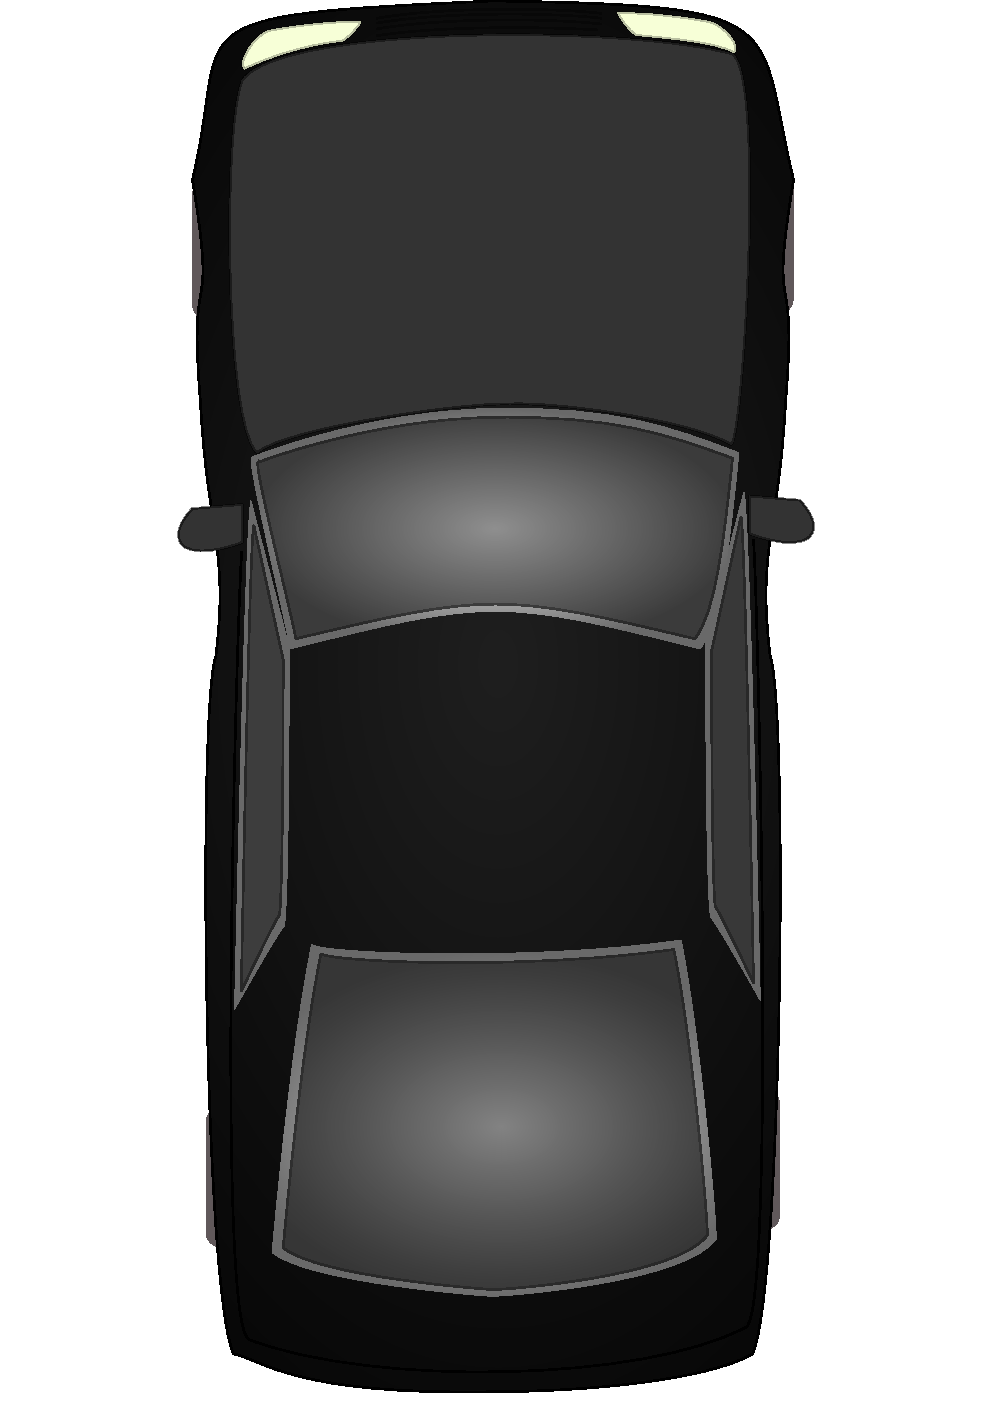
\includegraphics[width=2cm,angle=90,origin=c]{../deadlock/car-black.pdf}};
    },
    car black opposite rot/.pic={
        \node at (0,-0.25) {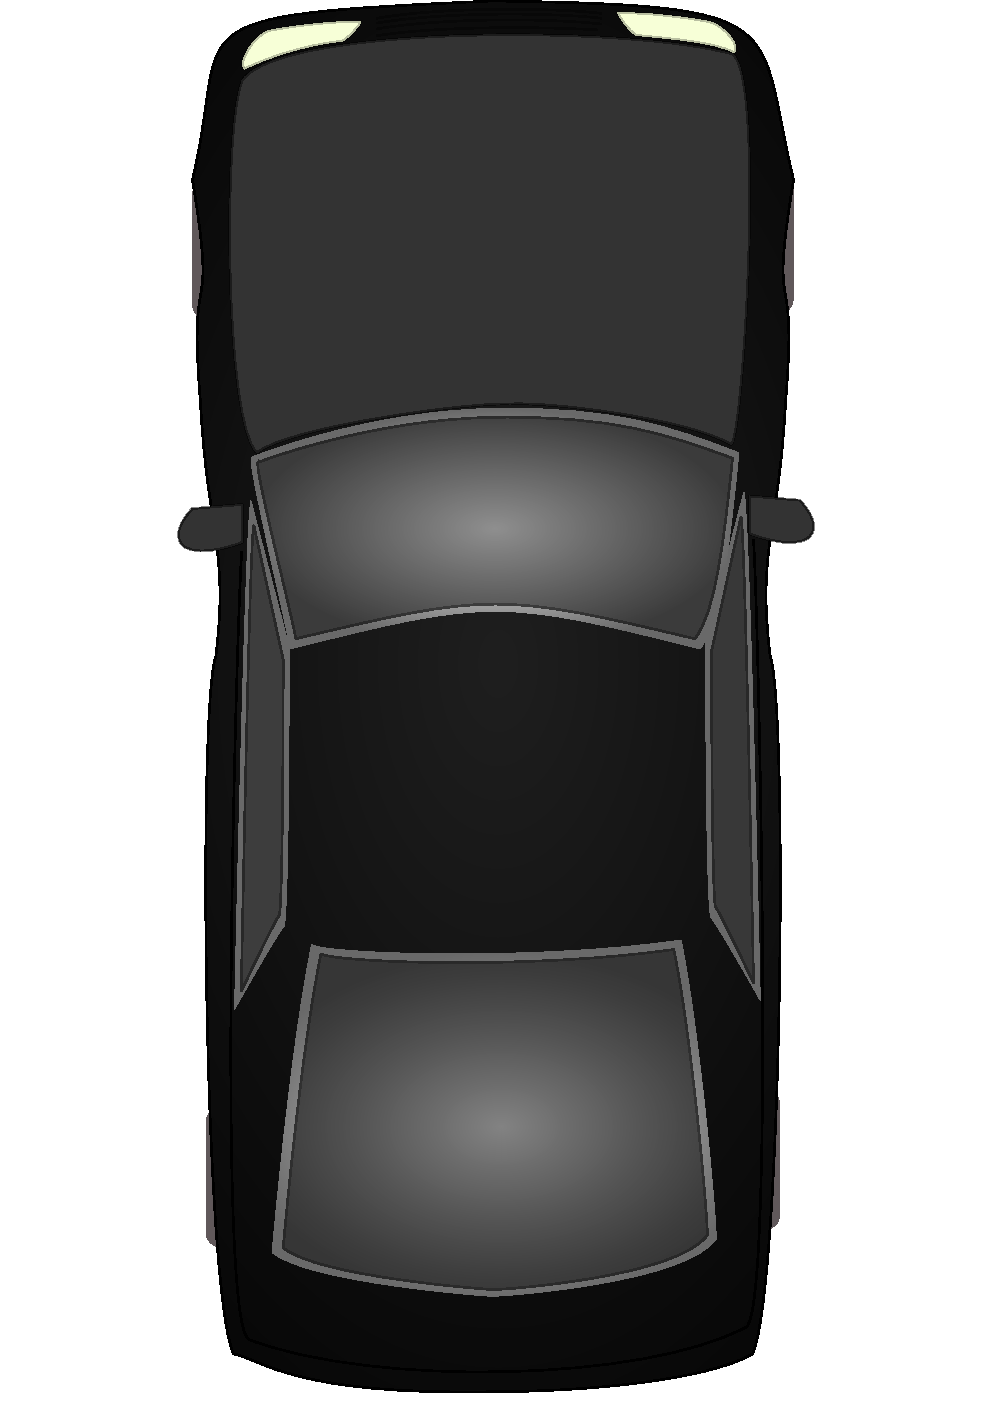
\includegraphics[width=2cm,angle=85,origin=c]{../deadlock/car-black.pdf}};
    },
    car yellow/.pic={
        \node at (0,-0.25) {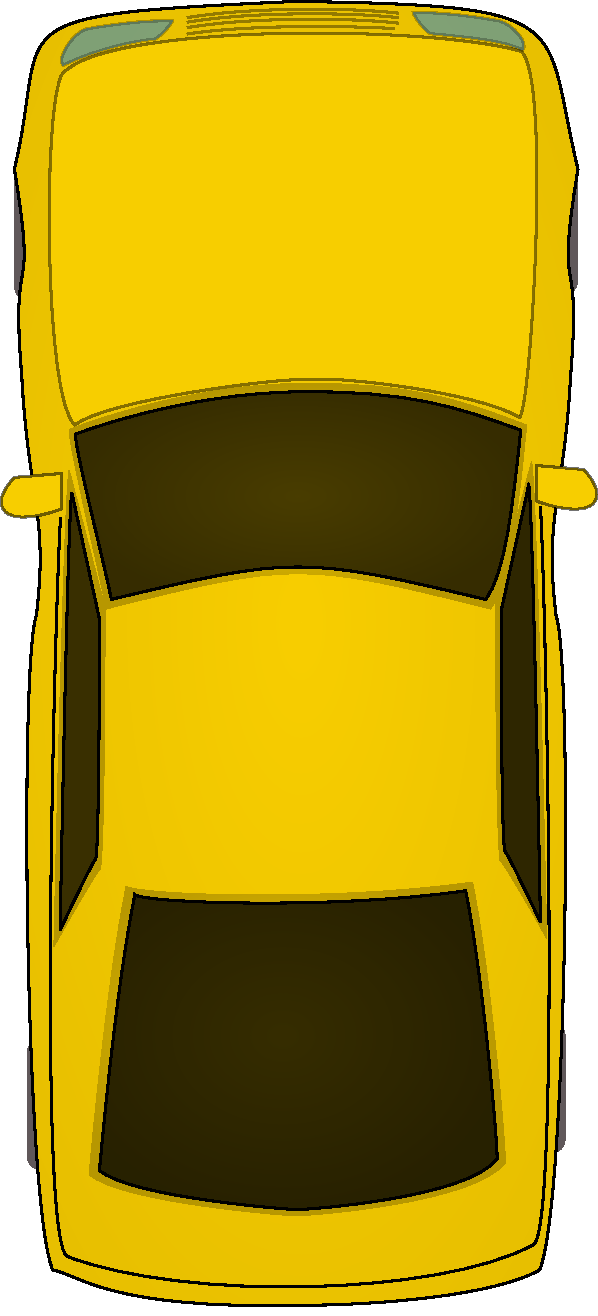
\includegraphics[width=1.25cm,angle=-90,origin=c]{../deadlock/car-yellow.pdf}};
    },
    car yellow rot/.pic={
        \node at (0,-0.25) {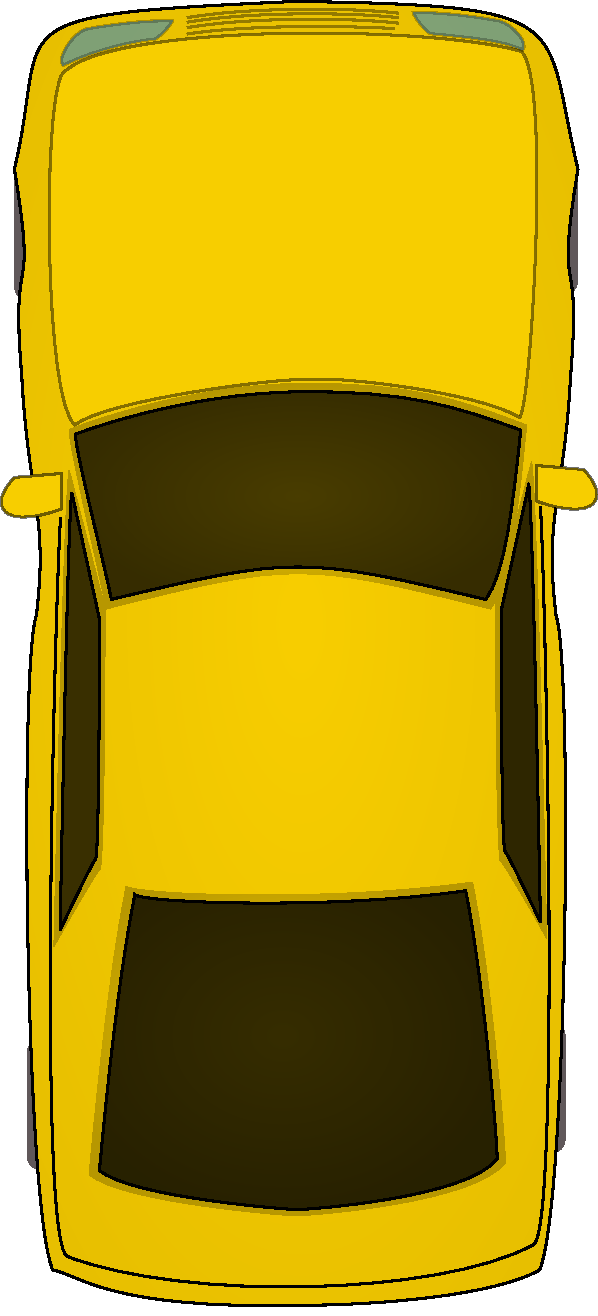
\includegraphics[width=1.25cm,angle=-100,origin=c]{../deadlock/car-yellow.pdf}};
    },
}
\draw[bridge line] (-4.5, -1) -- (-1, -1) -- (1, 0) -- (5, 0) -- (7, -1) -- (10.5, -1);
\draw[bridge line] (-4.5, 3) -- (-1, 3) -- (1, 2) -- (5, 2) -- (7, 3) -- (10.5, 3);
\draw[road divide] (-4.5, 1) -- (-1.5, 1);
\draw[road divide] (7.5, 1) -- (10.5, 1);

\begin{visibleenv}<1-2>
\path[overlay] (-3, 2) pic{car yellow};
\path[overlay] (9.5, 0) pic{car black opposite};
\end{visibleenv}

\begin{pgfonlayer}{bg}
\begin{visibleenv}<2>
\path[fill=yellow!60!black!20] (-1.5, 1) -- (-1.5, 3) -- (-1, 3) -- (1, 2) -- (2.5, 2) -- (2.5, 0) -- (1, 0) -- (-1, 1) -- cycle;
\end{visibleenv}
\begin{visibleenv}<2>
\path[fill=black!30] (8.0, 1) -- (8, -1) -- (7, -1) -- (5, 0) -- (4, 0) -- (4, 2) -- (5, 2) -- (7, 1) -- cycle;
\end{visibleenv}
\end{pgfonlayer}

\begin{visibleenv}<3-4>
\path[overlay] (1, 1.2) pic{car yellow rot};
\path[overlay] (5, 1) pic{car black opposite rot};
\end{visibleenv}

\end{tikzpicture}
\end{frame}
